\begin{figure}[H]
    \centering
    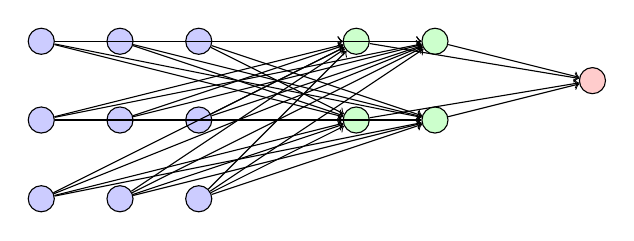
\begin{tikzpicture}
        \foreach \i in {0,1,2}
            \foreach \j in {0,1,2} {
                \node[circle, draw, fill=blue!20] (I\i\j) at (\i,\j) {};
            }
        \foreach \i in {0,1}
            \foreach \j in {0,1} {
                \node[circle, draw, fill=green!20] (C\i\j) at (\i+4,\j+1) {};
            }
        \node[circle, draw, fill=red!20] (FC) at (7,1.5) {};
        \foreach \i in {0,1,2}
            \foreach \j in {0,1,2} {
                \foreach \m in {0,1}
                    \foreach \n in {0,1} {
                        \draw[->] (I\i\j) -- (C\m\n);
                    }
            }
        \foreach \i in {0,1}
            \foreach \j in {0,1} {
                \draw[->] (C\i\j) -- (FC);
            }
    \end{tikzpicture}
    \caption{A simple convolutional neural network architecture.}
    \label{fig:cnn}
\end{figure}